\section{Approach} \label{approach}

In this section we discribe a modified skip-gram model that would better facilitate the embedding of words from source code than the normal skip-gram algorithm. We also discuss some preprocessing steps of the source code before using it as input. For the sake of simplicity and readability we will use Java as the example programming language during discussion for the rest of the paper. However, it should be noted that these ideas can be applied to any programming language with some modification.

\subsection{Preprocessing}

The source code will need to be preprocessed before being used in the skip-gram model. The main preprocessing step is the identification of the scope of variables and functions. For example, given a particular class in Java, a class variable can have the same name as a local variable. Similarly, two different classes may have the same function name. This is not a problem for natural language as every word in a natural language is unique. While having variables and functions with the same name is legal in Java (within certain rules), it can heavily skew the values of the word embeddings as all variables and functions with the same name will be mapped to the same word embedding. To account for this problem, we propose to extend all variable and function names with the class and function they belong to based on their scope. For example, given the Java class \textit{String}, its function \textit{charAt} will be extended to \textit{String.charAt}, and the local variable \textit{index} in the function \textit{charAt} will be extended to \textit{String.charAt.index}. This will ensure that all variable and function names are mapped to their own word embeddings.

However, this causes a new problem. If variable and function names are extended to be specific to the class they are defined in, then when analyzing new software there will be no word embeddings for any newly defined variables and functions. To remedy this, new software must first be input through the skip-gram model to produce the new necessary word embeddings before being input to a deep learning model.

Other preprocessing includes the removal of all unnecessary white space, some punctuation, and comments. We aknowledge that there are other possible preprocessing steps that can be taken, but we do not consider these at this time. For example, in Java it is legal to overload functions (that is, have different definitions and parameter lists for the same function name). We consider overloading the same as a word in natural language having multiple definitions. While the function is somewhat disambiguated, we believe it will not disambiguate enough to drastically change the results of a deep learning analysis.

\subsection{Modified Word2Vec}

As described earlier, Word2Vec uses a window size to determine the context of a word. This works fairly well for natural language processing because each word has a general predefined meaning and the syntax of a sentence does not allow for complex syntactic structures such as decision or loop statements. So a window size that only scans for context a bit before and after a word is able to determine a relative semantic meaning to other words. However, in source code variables and functions are defined within their class (and not always before they are used in the case of functions) and there are more complex syntactic structures. This seems to imply that a simple window size that scans before and after a word will not be sufficient in determining proper word embeddings for source code.

To modify skip-gram, we will need to separate ``key words'' (which includes key words, punctuation, and operands) from ``constructed words'' (which includes class, function, and variable names) defined in libraries or by programers. Key words are usually handled by the compiler and are not explicitly defined in a library, unlike the constructed words discussed later. We further divide key words into two categories, those that have a syntactic structure associated with them and those that do not. Such key words that have syntactic structures are \textit{if-else}, \textit{while}, \textit{for}, etc. These key words derive most of their meaning from their syntactic structure. Therefore, instead of using a window size, Word2Vec will consider everything that is a part of the structure as context when updating the word embedding values of that key word. For example, in the statements \textit{for(i; i $<$ 10; i++)\{ System.out.println(i); \}} everything between the parenthesis after the \textit{for} and before the \textit{\{} will be considered as context for the key word \textit{for}. It is important to note that we do not consider the statement within the loop structure (\textit{System.out.println(i);}) as part of the context for the key word \textit{for}, as the statements within key word syntactic structures do not usually have a direct impact on the meaning of the structure (and the key word associated with that structure). For the key words that do not have a syntactic structure (\textit{break}, \textit{+}, \textit{\&\&}, etc.), only context before and after the word is available to derive meaning. Therefore, Word2Vec will be used normally for these key words.

A constructed word's embedding will be use context in two separate ways. The first, and most important, is that word's definition. When a constructed word is defined, the entire definition is used as context to the skip-gram model. For example, for a Java class everything in the entire class is used as context; for a function, the function signature and entire definition will be used as context; for a variable, any assignment performed on it will be used as context. The second type of context will come from the constructed word's usage in code. In this case, Word2Vec will be used normally with a window size to capture code surrounding the word as context.

\begin{figure}
   \centering
   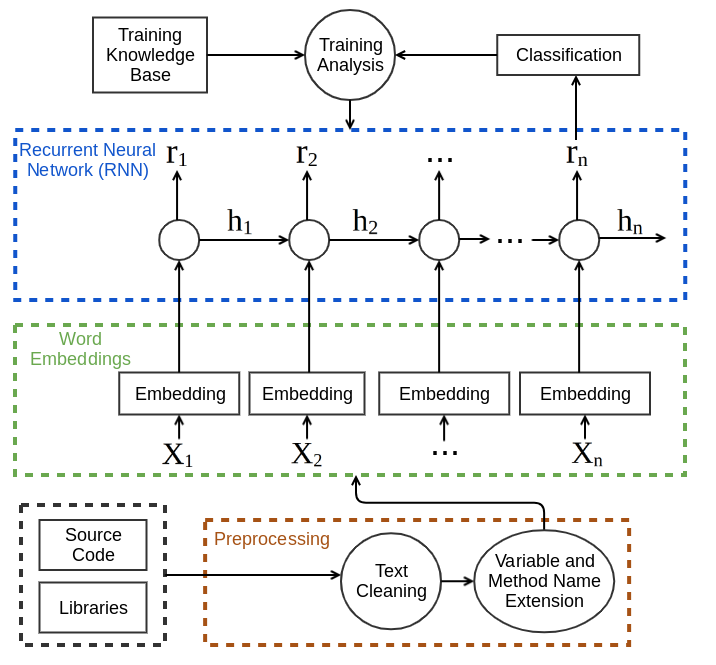
\includegraphics[scale=.32]{figures/deeplearningflow.png}
   \caption{Flow of Deep Learning Analysis}
   \label{deeplearningflow}
\end{figure}

\subsection{Deep Learning}

Once preprocessing and word embeddings have been completed, the source code is ready to be analyzed by a neural network. The network we will use is an RNN. This is appropriate since the current state of code at any time is dependent on what statements have been executed before it. Starting in the main function, for each word in the code, the embedding associated with that word will be used as input to the next step in the RNN. In the next section we will discuss how we plan to evaluate the effectiveness of deep learning on source code using the described approach.




